% Options for packages loaded elsewhere
\PassOptionsToPackage{unicode}{hyperref}
\PassOptionsToPackage{hyphens}{url}
\documentclass[
]{article}
\usepackage{xcolor}
\usepackage[margin=1in]{geometry}
\usepackage{amsmath,amssymb}
\setcounter{secnumdepth}{-\maxdimen} % remove section numbering
\usepackage{iftex}
\ifPDFTeX
  \usepackage[T1]{fontenc}
  \usepackage[utf8]{inputenc}
  \usepackage{textcomp} % provide euro and other symbols
\else % if luatex or xetex
  \usepackage{unicode-math} % this also loads fontspec
  \defaultfontfeatures{Scale=MatchLowercase}
  \defaultfontfeatures[\rmfamily]{Ligatures=TeX,Scale=1}
\fi
\usepackage{lmodern}
\ifPDFTeX\else
  % xetex/luatex font selection
\fi
% Use upquote if available, for straight quotes in verbatim environments
\IfFileExists{upquote.sty}{\usepackage{upquote}}{}
\IfFileExists{microtype.sty}{% use microtype if available
  \usepackage[]{microtype}
  \UseMicrotypeSet[protrusion]{basicmath} % disable protrusion for tt fonts
}{}
\makeatletter
\@ifundefined{KOMAClassName}{% if non-KOMA class
  \IfFileExists{parskip.sty}{%
    \usepackage{parskip}
  }{% else
    \setlength{\parindent}{0pt}
    \setlength{\parskip}{6pt plus 2pt minus 1pt}}
}{% if KOMA class
  \KOMAoptions{parskip=half}}
\makeatother
\usepackage{longtable,booktabs,array}
\usepackage{calc} % for calculating minipage widths
% Correct order of tables after \paragraph or \subparagraph
\usepackage{etoolbox}
\makeatletter
\patchcmd\longtable{\par}{\if@noskipsec\mbox{}\fi\par}{}{}
\makeatother
% Allow footnotes in longtable head/foot
\IfFileExists{footnotehyper.sty}{\usepackage{footnotehyper}}{\usepackage{footnote}}
\makesavenoteenv{longtable}
\usepackage{graphicx}
\makeatletter
\newsavebox\pandoc@box
\newcommand*\pandocbounded[1]{% scales image to fit in text height/width
  \sbox\pandoc@box{#1}%
  \Gscale@div\@tempa{\textheight}{\dimexpr\ht\pandoc@box+\dp\pandoc@box\relax}%
  \Gscale@div\@tempb{\linewidth}{\wd\pandoc@box}%
  \ifdim\@tempb\p@<\@tempa\p@\let\@tempa\@tempb\fi% select the smaller of both
  \ifdim\@tempa\p@<\p@\scalebox{\@tempa}{\usebox\pandoc@box}%
  \else\usebox{\pandoc@box}%
  \fi%
}
% Set default figure placement to htbp
\def\fps@figure{htbp}
\makeatother
\setlength{\emergencystretch}{3em} % prevent overfull lines
\providecommand{\tightlist}{%
  \setlength{\itemsep}{0pt}\setlength{\parskip}{0pt}}
\usepackage{amsmath,amssymb,mathtools,bm}
\usepackage[T1]{fontenc}
\usepackage{lmodern}
\usepackage{booktabs}
\usepackage{longtable}
\usepackage{array}
\usepackage{multirow}
\usepackage{wrapfig}
\usepackage{float}
\usepackage{colortbl}
\usepackage{pdflscape}
\usepackage{tabu}
\usepackage{threeparttable}
\usepackage{threeparttablex}
\usepackage[normalem]{ulem}
\usepackage{makecell}
\usepackage{xcolor}
\usepackage{bookmark}
\IfFileExists{xurl.sty}{\usepackage{xurl}}{} % add URL line breaks if available
\urlstyle{same}
\hypersetup{
  pdftitle={Statistics 520: Assignment 5},
  pdfauthor={Sam Olson},
  hidelinks,
  pdfcreator={LaTeX via pandoc}}

\title{Statistics 520: Assignment 5}
\author{Sam Olson}
\date{}

\begin{document}
\maketitle

\section{Assignment 5}\label{assignment-5}

The objectives of this assignment are to (1) ensure that you have a
grasp on using the tools of basic likelihood in a data analysis and (2)
help you to continue to develop the precise use of notation in
presenting descriptions of analyses. On the course web page is a file in
the Data folder called \texttt{gammadat.txt}. This file contains two
columns of values with a header having labels \texttt{group1} and
\texttt{group2}. Each column should be considered to contain values
corresponding to a set of independent and identical gamma random
variables. That is, the two columns are values from two groups that we
wish to compare using a two-sample model with gamma distributions.
Consider the first column to contain values for Group 1 and the second
column to contain values for Group 2.

A number of resources are available to you to help you complete this
assignment. Chapter 5 of the course notes contains a summary of
likelihood methods. In the Computing folder of the course web page is a
file \texttt{newtraph.txt} that contains a generic Newton-Raphson
algorithm that you may use for maximum likelihood estimation. There is
also a file called \texttt{newtraphexplain.txt} that describes the
inputs needed, the syntax, and the output. Alternatively you may choose
to make use of the built-in R functions \texttt{optim} or \texttt{nlm}.
Any of these options (or others you might know of if you prefer Matlab
or something else) are fine as long as you know what you are doing and
can produce the quantities needed to conduct the analysis.

Your answer should contain complete and consistent notation using no
undefined symbols. You should always clearly explain what you computed
and the formulas used. Your answer should not contain computer code or
material from a ``screen dump.'' You will not be awarded any points for
such material. If you want to report estimated values do so in the text,
as a list, or construct a table.

Again, do not include copied computer function output. You will not get
credit for anything presented in that way.

\newpage

\subsection{1.}\label{section}

Assume random variables \(Y_{1,1}, \ldots, Y_{1,n_1}\) and
\(Y_{2,1}, \ldots, Y_{2,n_2}\) have been defined for the responses in
this problem. These responses are strictly positive numbers, and an
assumption of independence is reasonable. Formulate a two-sample model
using gamma distributions. For one group, write the form of the log
likelihood that will need to be computed to find estimates and other
inferential quantities.

\subsubsection{Answer}\label{answer}

Assuming the random variables defined as given, taking observed values
that are strictly positive and iid.

Each group is then modeled with a (potentially different) Gamma
distribution parameterized by the (\(\alpha, \beta\)) parameters (shape
and rate, repectively):

\[
Y_{g,i}\;\stackrel{\text{iid}}{\sim}\;\mathrm{Gamma}(\alpha_g,\beta_g), \qquad g\in\{1,2\},\quad \text{and } i=1,\dots,n_g
\]

Where, for our purposes \(n_{1} = n_{2}\) (equal sample sizes between
the two groups of Gamma-distributed random variables).

With pdf of the form:

\[
f(y\mid \alpha_g,\beta_g)=\frac{\beta_g^{\alpha_g}}{\Gamma(\alpha_g)}\,y^{\alpha_g-1}e^{-\beta_g y},\qquad y>0,\;\alpha_g>0,\;\beta_g>0
\]

Using the pdf, we then take the log to define a single group \(g\)'s
log-likelihood function by:

\[
\ell_g(\alpha_g,\beta_g)
= \sum_{i=1}^{n_g}\log f(y_{g,i}\mid \alpha_g,\beta_g)
= n_g\Big(\alpha_g\log\beta_g-\log\Gamma(\alpha_g)\Big)
+(\alpha_g-1)\sum_{i=1}^{n_g}\log y_{g,i}
-\beta_g\sum_{i=1}^{n_g} y_{g,i}
\]

Note: The log-likelihood function is defined by 2 sufficient statistics,
of the form:

\[
T_{g,1}=\sum_{i=1}^{n_g}\log y_{g,i}
\quad\text{and}\quad
T_{g,2}=\sum_{i=1}^{n_g} y_{g,i}
\]

So, for the score equations, computing MLEs (say, via Newton--Raphson or
some other optimization methods) is done via:

\[
\frac{\partial \ell_g}{\partial \alpha_g}
= n_g\log \beta_g - n_g\psi_{0}(\alpha_g) + T_{g,1}, 
\qquad
\frac{\partial \ell_g}{\partial \beta_g}
= \frac{n_g\alpha_g}{\beta_g} - T_{g,2}
\]

With the Hessian given by:

\[
\frac{\partial^2 \ell_g}{\partial \alpha_g^2}
= -n_g \psi_{1}(\alpha_g),\qquad
\frac{\partial^2 \ell_g}{\partial \beta_g^2}
= -\frac{n_g\alpha_g}{\beta_g^2},\qquad
\frac{\partial^2 \ell_g}{\partial \alpha_g\,\partial \beta_g}
=\frac{n_g}{\beta_g}
\]

Giving the Hessian:

\[
\begin{bmatrix}
\displaystyle \frac{\partial^2 \ell_g}{\partial \alpha_g^2} &
\displaystyle \frac{\partial^2 \ell_g}{\partial \alpha_g \,\partial \beta_g} \\[1.2em]
\displaystyle \frac{\partial^2 \ell_g}{\partial \beta_g \,\partial \alpha_g} &
\displaystyle \frac{\partial^2 \ell_g}{\partial \beta_g^2}
\end{bmatrix}
=
\begin{bmatrix}
-\,n_g \psi_{1}(\alpha_g) & \tfrac{n_g}{\beta_g} \\[0.8em]
\tfrac{n_g}{\beta_g} & -\,\tfrac{n_g \alpha_g}{\beta_g^2}
\end{bmatrix}
\]

where \(\psi_{0}(\cdot)\) and \(\psi_{1}(\cdot)\) are the digamma and
trigamma functions, respectively (following notation convention seen on
Wikipedia).

Then, taking the individual group log-likelihoods, we calculate the full
two-sample log-likelihood as the sum (again, noting iid assumption
between and within groups):

\[
\begin{aligned}
\ell(\alpha_1,\beta_1,\alpha_2,\beta_2)
&= \ell_1(\alpha_1,\beta_1)+\ell_2(\alpha_2,\beta_2) \\ 
&= \sum_{g=1}^{2}\sum_{i=1}^{n_g}\log f(y_{g,i}\mid \alpha_g,\beta_g) \\ 
&= n_1\Big(\alpha_1\log\beta_1-\log\Gamma(\alpha_1)\Big)
+(\alpha_1-1)\sum_{i=1}^{n_1}\log y_{1,i}
-\beta_1\sum_{i=1}^{n_1} y_{1,i} \\ 
&+ n_2\Big(\alpha_2\log\beta_2-\log\Gamma(\alpha_2)\Big)
+(\alpha_2-1)\sum_{j=1}^{n_2}\log y_{2,j}
-\beta_2\sum_{j=1}^{n_2} y_{2,j} \\
\end{aligned}
\]

\newpage

\subsection{2.}\label{section-1}

Find maximum likelihood estimates and 95\% Wald theory intervals for the
parameters of each group. Recall that, in the data file, the first
column of values is Group 1 and the second column of values is Group 2.

\subsubsection{Answer}\label{answer-1}

As noted in part 1)., the log-likelihood is of the form:

\[
\ell_g(\alpha_g,\beta_g)
= n_g\big(\alpha_g\log\beta_g-\log\Gamma(\alpha_g)\big)
 +(\alpha_g-1)\sum_{i=1}^{n_g}\log Y_{g,i}
 -\beta_g\sum_{i=1}^{n_g}Y_{g,i} \quad \text{where } g \in \{1, 2\}
\]

Setting the score functions to zero gives the standard MLE system of
equations.

The Fisher Information (negative of the Hessian of the log-likelihood
evaluated at the MLE, \((\alpha_g,\beta_g)\)) then is:

\[
I_g(\alpha_g,\beta_g)=
\begin{pmatrix}
n_g\,\psi_{1}(\alpha_g) & -\,n_g/\beta_g\\[4pt]
-\,n_g/\beta_g & n_g\,\alpha_g/\beta_g^2
\end{pmatrix}
\]

Taking these quantities, the Wald covariance is then given by:

\[
\widehat{\mathrm{Var}}\!\begin{pmatrix}\hat\alpha_g\\ \hat\beta_g\end{pmatrix}
= I_g(\hat\alpha_g,\hat\beta_g)^{-1}
\]

After numeric approximation, taking square roots where appropriate
(square root of the variance is SE), and evaluating the typical
expression for confidence intervals, we have (with each group having
\(n_1=n_2=50\) samples):

\begin{longtable}[]{@{}
  >{\raggedright\arraybackslash}p{(\linewidth - 12\tabcolsep) * \real{0.0521}}
  >{\raggedleft\arraybackslash}p{(\linewidth - 12\tabcolsep) * \real{0.1250}}
  >{\raggedleft\arraybackslash}p{(\linewidth - 12\tabcolsep) * \real{0.1667}}
  >{\raggedright\arraybackslash}p{(\linewidth - 12\tabcolsep) * \real{0.1979}}
  >{\raggedleft\arraybackslash}p{(\linewidth - 12\tabcolsep) * \real{0.1146}}
  >{\raggedleft\arraybackslash}p{(\linewidth - 12\tabcolsep) * \real{0.1562}}
  >{\raggedright\arraybackslash}p{(\linewidth - 12\tabcolsep) * \real{0.1875}}@{}}
\toprule\noalign{}
\begin{minipage}[b]{\linewidth}\raggedright
Group
\end{minipage} & \begin{minipage}[b]{\linewidth}\raggedleft
\(\hat\alpha\)
\end{minipage} & \begin{minipage}[b]{\linewidth}\raggedleft
SE(\(\hat\alpha\))
\end{minipage} & \begin{minipage}[b]{\linewidth}\raggedright
95\% CI for \(\alpha\)
\end{minipage} & \begin{minipage}[b]{\linewidth}\raggedleft
\(\hat\beta\)
\end{minipage} & \begin{minipage}[b]{\linewidth}\raggedleft
SE(\(\hat\beta\))
\end{minipage} & \begin{minipage}[b]{\linewidth}\raggedright
95\% CI for \(\beta\)
\end{minipage} \\
\midrule\noalign{}
\endhead
\bottomrule\noalign{}
\endlastfoot
1 & 3.497 & 0.669 & (2.186, 4.808) & 1.519 & 0.312 & (0.907, 2.131) \\
2 & 1.626 & 0.298 & (1.042, 2.210) & 0.726 & 0.155 & (0.421, 1.031) \\
\end{longtable}

Note, to be explicit about the formula for confidence intervals:

\[
\exp \left( \log \hat\alpha \;\pm\; z_{1-\gamma/2}\,\mathrm{SE}(\log \hat\alpha) \right) \quad \text{ and } \exp \left( \log \hat\beta \;\pm\; z_{1-\gamma/2}\,\mathrm{SE}(\log \hat\beta) \right)
\]

Where \(\gamma = 0.05, 1- \frac{\gamma}{2} = 0.975\)

And to be explicit about the optimization method used: Using R's
\texttt{optim} function for maximization (minimize negative
log-likelihood), which is a ``quasi-Newton method'', i.e., using the
original log-likelihood, first derivative, and second derivative (also
using \texttt{method\ =\ ‘BFGS’}).

\newpage

\subsection{3.}\label{section-2}

Using a likelihood ratio test, determine whether you would reject a
model having a common gamma distribution for both groups in favor of a
model having separate gamma distributions for each of the two groups.
Produce a plot of the estimated densities for each group (both densities
on the same plot).

\subsubsection{Answer}\label{answer-2}

Define the (nested) hypotheses by:

\begin{itemize}
\tightlist
\item
  \(H_0:\) \(\alpha_1=\alpha_2\) and \(\beta_1=\beta_2\) (one common
  Gamma for both groups, only 2 unique parameters between groups).
\item
  \(H_1:\) \((\alpha_1 \neq \alpha_2)\) and \((\beta_1 \neq \beta_2)\)
  (two separate Gammas, 4 unique parameters between groups).
\end{itemize}

Let \(\hat\theta_0=(\hat\alpha_0,\hat\beta_0)\) be the MLE under \(H_0\)
(fitted using pooled data), and
\(\hat\theta_1=((\hat\alpha_1,\hat\beta_1),(\hat\alpha_2,\hat\beta_2))\)
the MLEs fitted to each group separately.

The LRT statistic is of the form:

\[
\Lambda = - 2\bigl\{\ell(\hat\theta_0) - \ell(\hat\theta_1)\bigr\}
\;\xrightarrow{d}\; \chi^2_{\,2}
\]

With degrees of freedom 2 from (full - reduced = 4 - 2), i.e., \(H_1\)
has two more ``free'' parameters than \(H_0\).

Using the same optimization method using in part 2., we calculate:

\begin{itemize}
\item
  Separate-group MLEs: \(\hat\alpha_1=3.497,\;\hat\beta_1=1.519\), and
  \(\hat\alpha_2=1.626,\;\hat\beta_2=0.726\)
\item
  Common (pooled) MLEs: \(\hat\alpha_0=2.202,\;\hat\beta_0=0.970\)
\end{itemize}

Where:

\[
\ell(\hat\theta_1)=-163.447 (= \ell_1(\alpha_1,\beta_1)+\ell_2(\alpha_2,\beta_2) = -76.22814 + -87.21866),\qquad \ell(\hat\theta_0)=-167.526
\]

Using the log-likelihood values above, the LRT statistic is:

\[
\Lambda = - 2 (- 167.526 - (-163.447)) = 8.158
\]

With corresponding p-value (with reference distribution \(\chi^2_2\):

\[
p\text{-value} = 0.01693 
\]

Reducing the question to an ``Accept''/``Reject'' framework, we Reject
\(H_0\) at the \(\alpha = 0.05\) level (or make a ``strength of
evidence'' argument to say we have strong evidence in favor of rejecting
the null hypothesis). Interpreting this, we'd say that modeling the two
groups as separate (differently parametrized) Gamma distributions seems
a better fit than pooling them together as a single Gamma distribution
(with shared shape and rate parameters).

And a graph!

\pandocbounded{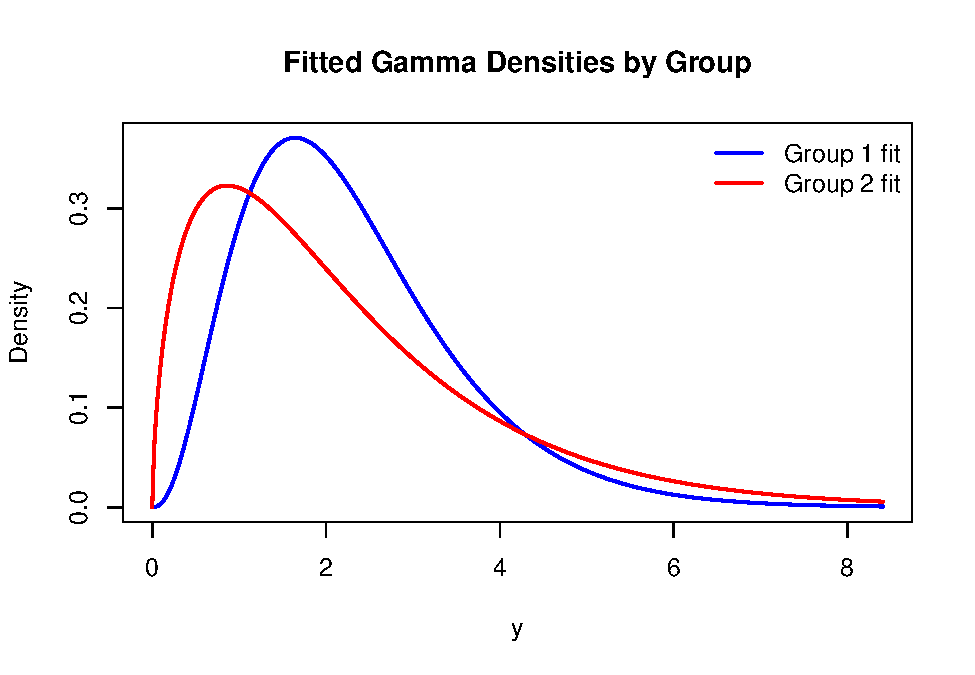
\includegraphics[keepaspectratio]{HW5_files/figure-latex/unnamed-chunk-4-1.pdf}}

\newpage

\subsection{4.}\label{section-3}

Find maximum likelihood estimates and 95\% Wald theory intervals for the
expected value of each group. Also produce a 95\% interval for the
difference in expected values (Group 1 minus Group 2).

\subsubsection{Answer}\label{answer-3}

For a Gamma distributed random variable Y, whose distribution is
parametrized by the shape and rate parameters, the expected value is of
the form:

\[
E[Y] = \frac{\alpha}{\beta}
\]

For our case, thus the expected values for each group are given by:

\[
\mu_g = \frac{\alpha_g}{\beta_g},\qquad g=1,2
\]

Let \((\hat\alpha_g,\hat\beta_g)\) be the MLEs, then:

\[
\hat{\mu_g} = \frac{\hat{\alpha_g}}{\hat{\beta_g}},\qquad g=1,2
\]

Note then that the covariance matrix of the MLEs (the inverse observed
information) is given by:

\[
\widehat\Sigma_g = \begin{bmatrix}\widehat{\mathrm{Var}}(\hat\alpha_g) & \widehat{\mathrm{Cov}}(\hat\alpha_g,\hat\beta_g)\\ \widehat{\mathrm{Cov}}(\hat\alpha_g,\hat\beta_g) & \widehat{\mathrm{Var}}(\hat\beta_g)\end{bmatrix}
\]

Then, using the delta method with gradient given by:

\[
\begin{aligned}
\nabla\mu_g(\alpha,\beta) 
&= (\frac{\partial}{\partial \alpha} (\hat{\mu_g}), \frac{\partial}{\partial \beta} (\hat{\mu_g})) \\ 
&= (\frac{\partial}{\partial \alpha} (\frac{\hat{\alpha_g}}{\hat{\beta_g}}), \frac{\partial}{\partial \beta} (\frac{\hat{\alpha_g}}{\hat{\beta_g}})) \\ 
&= \left(\tfrac{1}{\beta},\; -\tfrac{\alpha}{\beta^2}\right) \\ 
\end{aligned}
\]

Then

\[
\widehat{\mathrm{Var}}(\hat\mu_g)
= \nabla\mu_g^\top \,\widehat\Sigma_g \,\nabla\mu_g
\]

Taking the SE then is just taking the root of the above quantity.

Note: When calculating the quantities of interest, we use the sample
(observed) variances of \(\hat{\alpha}\) and \(\hat{\beta}\).

Then, we may construct a 95\% Wald interval for \(\mu_g\) by:

\[
\hat\mu_g \pm z_{1 - \frac{\gamma}{2}} \mathrm{SE}(\hat\mu_g)
= \hat\mu_g \pm 1.96\,\mathrm{SE}(\hat\mu_g)
\]

(Using 1.96 based on the Standard Normal distribution, where
\(\gamma = 0.05\), as Wald Theory uses asymptotic results.)

\newpage

For the difference \(\mu_1-\mu_2\), treat groups as independent, i.e.,
\(\mathrm{Cov}(\hat{\mu_1}, \hat{\mu_2}) = 0\), so

\[
\begin{aligned}
\widehat{\mathrm{Var}}(\hat\mu_1-\hat\mu_2)
&= \widehat{\mathrm{Var}}(\hat\mu_1)+\widehat{\mathrm{Var}}(\hat\mu_2) + 2\widehat{\mathrm{Cov}}(\hat{\mu_1}, \hat{\mu_2})\\
&= \widehat{\mathrm{Var}}(\hat\mu_1)+\widehat{\mathrm{Var}}(\hat\mu_2) \\ 
\end{aligned}
\]

Taken together, the quantities of interest we estimate are:

\begin{longtable}[]{@{}lrrrr@{}}
\caption{Gamma means and 95\% Wald intervals}\tabularnewline
\toprule\noalign{}
group & mu\_hat & se & ci\_L & ci\_U \\
\midrule\noalign{}
\endfirsthead
\toprule\noalign{}
group & mu\_hat & se & ci\_L & ci\_U \\
\midrule\noalign{}
\endhead
\bottomrule\noalign{}
\endlastfoot
group1 & 2.302 & 0.174 & 1.961 & 2.644 \\
group2 & 2.240 & 0.248 & 1.753 & 2.726 \\
difference (1 - 2) & 0.063 & 0.303 & -0.532 & 0.657 \\
\end{longtable}

\newpage

\subsection{5.}\label{section-4}

Test whether the two groups should be considered significantly different
using a two-sample \(t\)-test. (Take square roots if you think it makes
the data look more symmetric for each group, though this is optional.)
Does your result agree with the likelihood ratio test? Does it agree
with the interval for difference in expected values?

\subsubsection{Answer}\label{answer-4}

The observed group sample means are given by:

\begin{itemize}
\item
  Group 1: \(\bar y_1 \approx 2.29\) (2.30 expected),
\item
  Group 2: \(\bar y_2 \approx 2.24\) (2.24 expected).
\end{itemize}

Also, the observed sample standard deviation is given by.

\begin{itemize}
\item
  Group 1: \(s_1 \approx 1.31\)
\item
  Group 2: \(s_2 \approx 1.75\)
\item
  Pooled: \(s_0 \approx 1.55\)
\end{itemize}

And we have equal number of samples per group, \(n_1=n_2=50\), which
taken together could justify use of the two-sample t-test.

The hypotheses we may then test are o the form:

\[
H_0:\; \mu_1=\mu_2 \quad\text{vs.}\quad H_A:\; \mu_1\ne \mu_2
\]

Since there are differences in variance between Group 1 and Group 2, I
used the Welch two-sample \(t\)-test (which does not assume equal
variances between groups). Notably, while I cannot emphatically justify
using Welch, I prefer to use it in this instance because it reduces to
the (``pooled'') two-sample \(t\)-test when the sample variances are
close (which I think they are, though still distinct between groups).

Additionally: While the formulas below are for the Welch two-sample
\(t\)-test, I also calculate and provide formulas for the (non-Welch,
standard) two-sample \(t\)-test.

That being said, the relevant formulas for the Welch are of the form:

\[
t_{\nu} = \frac{\bar y_1-\bar y_2}{\sqrt{s_1^2/n_1 + s_2^2/n_2}} \approx 0.15
\]

Where the degrees of freedom are calculated using the
Welch-Satterthwaite approximation:

\[
\nu \;=\; 
\frac{\left(\dfrac{s_1^2}{n_1} + \dfrac{s_2^2}{n_2}\right)^{2}}
{\dfrac{\left(\dfrac{s_1^2}{n_1}\right)^{2}}{n_1 - 1} \;+\; \dfrac{\left(\dfrac{s_2^2}{n_2}\right)^{2}}{n_2 - 1}}
\]

The corresponding p-value is then: \(p\approx 0.84\) (using Welch, and
with no transformation).

If we repeat this process \emph{after} doing a \texttt{sqrt}
transformation on the observed samples, the result is very similar: The
test statistic is \(t_{98} \approx 0.78\) with corresponding
\(p \approx 0.44\) (again, using Welch). So, reducing to a decision
``Accept''/``Reject'' or even a ``strength of evidence'' argument, the
interpretation remains largely the same.

These results may (at first) seem opposed to the Likelihood ratio test
from part 3), but it isn't. Importantly, these two methods (LRT test
vs.~the two-sample t-test) correspond to different tests. The two-sample
\(t\)-test does not provide evidence of a significant difference in
means between the two groups. This is also consistent with the Wald
interval for the difference in means \(\mu_1-\mu_2\), containing 0. But
LRT is not a direct comparison of means; instead, the LRT tests whether
the two \emph{distributions} (particularly, the parameters and
distributional form, so encompassing distributional shape, spread, and
other aspects of the distributional form) differ significantly between
groups.

Also, the results of the two-sample test are consistent when we use the
normal ``pooled'' two-sample t-test, and also when we transform the
original data using the \texttt{sqrt} transformation. All the relevant
statistics and summary information of the calculations considered are in
the following table:

\begin{longtable}[]{@{}
  >{\raggedright\arraybackslash}p{(\linewidth - 18\tabcolsep) * \real{0.1688}}
  >{\raggedleft\arraybackslash}p{(\linewidth - 18\tabcolsep) * \real{0.0779}}
  >{\raggedleft\arraybackslash}p{(\linewidth - 18\tabcolsep) * \real{0.0779}}
  >{\raggedleft\arraybackslash}p{(\linewidth - 18\tabcolsep) * \real{0.0779}}
  >{\raggedleft\arraybackslash}p{(\linewidth - 18\tabcolsep) * \real{0.0779}}
  >{\raggedleft\arraybackslash}p{(\linewidth - 18\tabcolsep) * \real{0.0909}}
  >{\raggedleft\arraybackslash}p{(\linewidth - 18\tabcolsep) * \real{0.0909}}
  >{\raggedleft\arraybackslash}p{(\linewidth - 18\tabcolsep) * \real{0.1039}}
  >{\raggedleft\arraybackslash}p{(\linewidth - 18\tabcolsep) * \real{0.1169}}
  >{\raggedleft\arraybackslash}p{(\linewidth - 18\tabcolsep) * \real{0.1169}}@{}}
\caption{Table of Two-Sample Test Statistics}\tabularnewline
\toprule\noalign{}
\begin{minipage}[b]{\linewidth}\raggedright
analysis
\end{minipage} & \begin{minipage}[b]{\linewidth}\raggedleft
mean1
\end{minipage} & \begin{minipage}[b]{\linewidth}\raggedleft
mean2
\end{minipage} & \begin{minipage}[b]{\linewidth}\raggedleft
sd1
\end{minipage} & \begin{minipage}[b]{\linewidth}\raggedleft
sd2
\end{minipage} & \begin{minipage}[b]{\linewidth}\raggedleft
t\_stat
\end{minipage} & \begin{minipage}[b]{\linewidth}\raggedleft
df
\end{minipage} & \begin{minipage}[b]{\linewidth}\raggedleft
p\_value
\end{minipage} & \begin{minipage}[b]{\linewidth}\raggedleft
ci\_lower
\end{minipage} & \begin{minipage}[b]{\linewidth}\raggedleft
ci\_upper
\end{minipage} \\
\midrule\noalign{}
\endfirsthead
\toprule\noalign{}
\begin{minipage}[b]{\linewidth}\raggedright
analysis
\end{minipage} & \begin{minipage}[b]{\linewidth}\raggedleft
mean1
\end{minipage} & \begin{minipage}[b]{\linewidth}\raggedleft
mean2
\end{minipage} & \begin{minipage}[b]{\linewidth}\raggedleft
sd1
\end{minipage} & \begin{minipage}[b]{\linewidth}\raggedleft
sd2
\end{minipage} & \begin{minipage}[b]{\linewidth}\raggedleft
t\_stat
\end{minipage} & \begin{minipage}[b]{\linewidth}\raggedleft
df
\end{minipage} & \begin{minipage}[b]{\linewidth}\raggedleft
p\_value
\end{minipage} & \begin{minipage}[b]{\linewidth}\raggedleft
ci\_lower
\end{minipage} & \begin{minipage}[b]{\linewidth}\raggedleft
ci\_upper
\end{minipage} \\
\midrule\noalign{}
\endhead
\bottomrule\noalign{}
\endlastfoot
Raw, Welch & 2.302 & 2.240 & 1.308 & 1.755 & 0.203 & 90.608 & 0.840 &
-0.552 & 0.678 \\
Sqrt, Welch & 1.463 & 1.386 & 0.406 & 0.571 & 0.781 & 88.471 & 0.437 &
-0.119 & 0.274 \\
Raw, pooled & 2.302 & 2.240 & 1.308 & 1.755 & 0.203 & 98.000 & 0.840 &
-0.552 & 0.677 \\
Sqrt, pooled & 1.463 & 1.386 & 0.406 & 0.571 & 0.781 & 98.000 & 0.436 &
-0.119 & 0.274 \\
\end{longtable}

Misc: There are two notes to the above. First is, the Welch seemed most
appropriate given differences in variance (and differences in shape-rate
parameters), hence why it was formally noted and used. However, since
the two-sample t-test was also calculated, the formulas used are as
follows:

\[
s_p^2 \;=\; \frac{(n_1-1)s_1^2 + (n_2-1)s_2^2}{\,n_1+n_2-2\,} 
\]

\[
t_{df} \;=\; \frac{\bar{y}_1 - \bar{y}_2}{s_p \sqrt{\tfrac{1}{n_1} + \tfrac{1}{n_2}}},
\qquad \text{df} = n_1+n_2-2
\]

Where \(\text{df}, s_p^2,  \text{ and } t_P\) as given in the above
table.

Also, since I included the \texttt{sqrt} evaluation as well in the
table, below is visual evidence that the distributions appear more
symmetric after \texttt{sqrt} transformation to the data (which also
gives further visual evidence of the spread/variance being different
between the two groups).

\pandocbounded{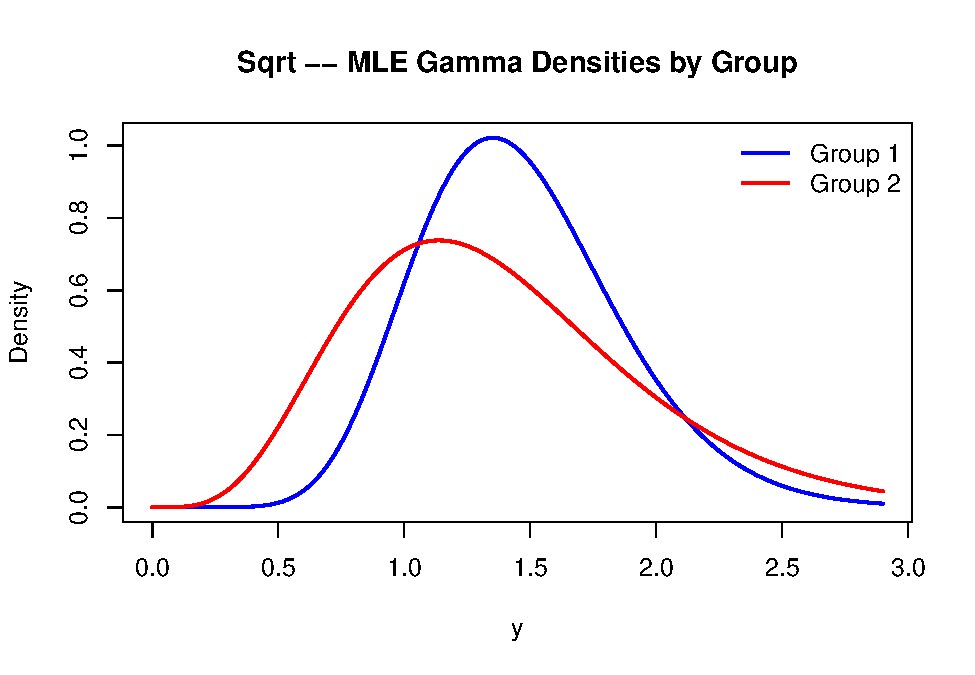
\includegraphics[keepaspectratio]{HW5_files/figure-latex/unnamed-chunk-10-1.pdf}}

\newpage

\subsection{6.}\label{section-5}

Find maximum likelihood estimates and 95\% Wald theory intervals for the
mode of each group. Also produce a 95\% interval for the difference in
modes (Group 1 minus Group 2).

\subsubsection{Answer}\label{answer-5}

For Y a Gamma-distributed random variable, parametrized in shape--rate
form, the mode is of the form:

\[
\text{mode} =
\begin{cases}
\dfrac{\alpha-1}{\beta}, & \alpha>1,\\[6pt]
0, & 0 < \alpha\le 1\ 
\end{cases}
\]

As the MLEs of \(\hat{\alpha_1}, \hat{\alpha_2} > 1\), we won't worry
about the second condition of the mode, i.e., where
\(0 < \alpha \leq 1\).

As defined previously, \((\hat\alpha_g,\hat\beta_g)\) are the MLEs for
group \(g\) with covariance given by \(\widehat\Sigma_g\).

For \(\hat\alpha_g>1\), we use the delta method with the expressions:

\[
m_g(\alpha,\beta)=\frac{\alpha-1}{\beta},\qquad 
\nabla m_g(\alpha,\beta)=\Big(\tfrac{1}{\beta},\ -\tfrac{\alpha-1}{\beta^2}\Big)
\]

Again, mirroring the formulae used in part 4).

We then have the quantities:

\[
\widehat{\mathrm{Var}}(\hat m_g)=\nabla m_g^\top\,\widehat\Sigma_g\,\nabla m_g,\qquad
\text{SE}(\hat m_g)=\sqrt{\widehat{\mathrm{Var}}(\hat m_g)}
\]

To construct a 95\% Wald CI, given by:

\[
\hat m_g \pm z_{1 - \frac{\gamma}{2}} \,\text{SE}(\hat m_g) =
\hat m_g \pm 1.96\,\text{SE}(\hat m_g)
\]

For the difference \(m_1-m_2\), independence of groups gives

\[
\begin{aligned}
\widehat{\mathrm{Var}}(\hat{m_1}-\hat{m_2})
&= \widehat{\mathrm{Var}}(\hat{m_1})+\widehat{\mathrm{Var}}(\hat{m_2}) + 2\widehat{\mathrm{Cov}}(\hat{m_1}, \hat{m_2})\\
&= \widehat{\mathrm{Var}}(\hat{m_1})+\widehat{\mathrm{Var}}(\hat{m_2}) \\ 
\end{aligned}
\]

Calculating these quantities gives us the following table:

\begin{longtable}[]{@{}lrrrr@{}}
\caption{Gamma modes and 95\% Wald intervals}\tabularnewline
\toprule\noalign{}
group & mode\_hat & se & ci\_L & ci\_U \\
\midrule\noalign{}
\endfirsthead
\toprule\noalign{}
group & mode\_hat & se & ci\_L & ci\_U \\
\midrule\noalign{}
\endhead
\bottomrule\noalign{}
\endlastfoot
group1 & 1.644 & 0.177 & 1.297 & 1.991 \\
group2 & 0.862 & 0.270 & 0.334 & 1.391 \\
difference (1 - 2) & 0.782 & 0.323 & 0.149 & 1.414 \\
\end{longtable}

\newpage

\subsection{7.}\label{section-6}

Although model assessment has not yet been covered formally, it is
intuitive that the estimated distribution function (CDF) under our model
and the empirical distribution function of the data should be similar.
Produce plots of the estimated distribution function for each group with
the empirical distribution function overlaid.

\subsubsection{Answer}\label{answer-6}

To avoid any potential ``code dump'' regarding this question, I just
wanted to note that the \texttt{stats} package contains an \texttt{ecdf}
function. This was used for the following comparisons with the
``expected'' line (based on the MLEs \(\hat{\alpha_g}, \hat{\beta_g}\),
\(g \in \{1, 2 \}\)).

\pandocbounded{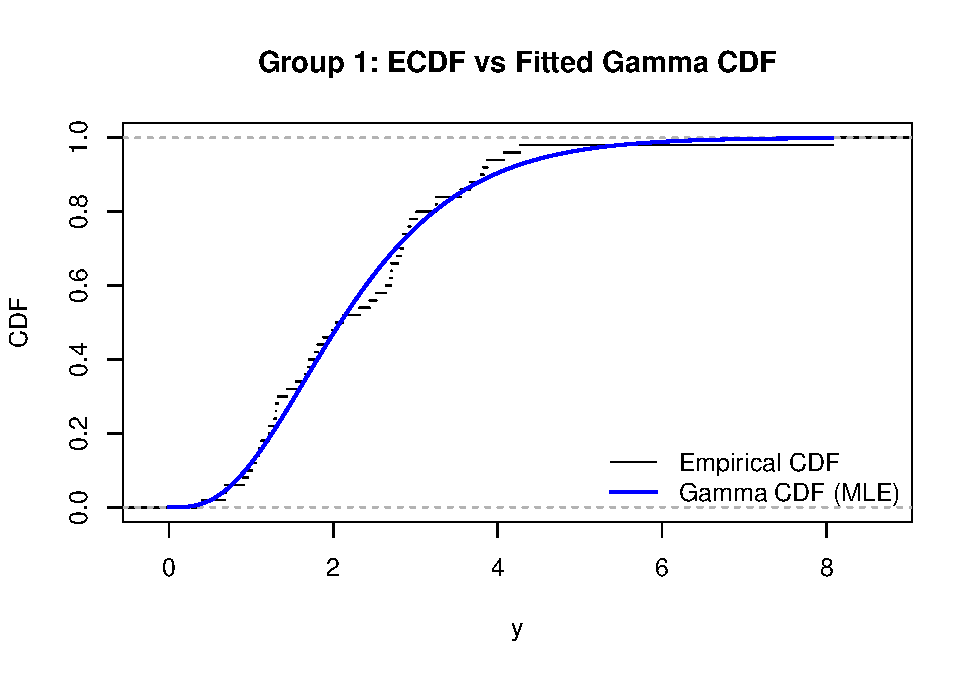
\includegraphics[keepaspectratio]{HW5_files/figure-latex/unnamed-chunk-12-1.pdf}}

\newpage

\subsection{8.}\label{section-7}

Write a short paragraph giving your conclusions about this group
comparison.

\subsubsection{Answer}\label{answer-7}

Comparing the ECDFs to their fitted Gamma distributions, both groups
match reasonably well, although Group 1 has more visually apparent
differences in the 2--4 range (domain). In terms of expectation/central
tendency, the two groups have very similar means, as evidenced when
comparing means via the two-sample t-tests. It is then perhaps
unsurprising that the Wald confidence interval for the difference in
expected values includes zero. However, the likelihood ratio test
provides some evidence that the overall distributions differ, with Group
1 and Group 2 having distinct shape--rate parameter combinations (their
individual parameter values). This is also evidenced somewhat in the
above visual, as the ECDFs and fitted Gamma CDFs look different between
the two groups. To put it hopefully succinctly: The results from the
prior parts (1 through 7) suggest that while the groups do not differ
significantly in their means, their distributional shapes are different
enough to warrant modeling them separately.

\end{document}
